%%%%%%%%%%%%%%%%%%%%%%%%%%%%%%%%%%%%%%%%%
% Programming/Coding Assignment
% LaTeX Template
%
% This template has been downloaded from:
% http://www.latextemplates.com
%
% Original author:
% Ted Pavlic (http://www.tedpavlic.com)
%
% Note:
% The \lipsum[#] commands throughout this template generate dummy text
% to fill the template out. These commands should all be removed when 
% writing assignment content.
%
% This template uses a Perl script as an example snippet of code, most other
% languages are also usable. Configure them in the "CODE INCLUSION 
% CONFIGURATION" section.
%
%Assignment 1
%Author Zetan
%%%%%%%%%%%%%%%%%%%%%%%%%%%%%%%%%%%%%%%%%

%----------------------------------------------------------------------------------------
%	PACKAGES AND OTHER DOCUMENT CONFIGURATIONS
%----------------------------------------------------------------------------------------

\documentclass{article}

\usepackage{fancyhdr} % Required for custom headers
\usepackage{lastpage} % Required to determine the last page for the footer
\usepackage{extramarks} % Required for headers and footers
\usepackage[usenames,dvipsnames]{color} % Required for custom colors
\usepackage{graphicx} % Required to insert images
\usepackage{listings} % Required for insertion of code
\usepackage{courier} % Required for the courier font
\usepackage{lipsum} % Used for inserting dummy 'Lorem ipsum' text into the template
\usepackage{url}

% Margins
\topmargin=-0.45in
\evensidemargin=0in
\oddsidemargin=0in
\textwidth=6.5in
\textheight=9.0in
\headsep=0.25in

\linespread{1.1} % Line spacing

% Set up the header and footer
\pagestyle{fancy}
\lhead{\hmwkAuthorName} % Top left header
\chead{\hmwkClass\ (\hmwkClassInstructor\ \hmwkClassTime): \hmwkTitle} % Top center head
\rhead{\firstxmark} % Top right header
\lfoot{\lastxmark} % Bottom left footer
\cfoot{} % Bottom center footer
\rfoot{Page\ \thepage\ of\ \protect\pageref{LastPage}} % Bottom right footer
\renewcommand\headrulewidth{0.4pt} % Size of the header rule
\renewcommand\footrulewidth{0.4pt} % Size of the footer rule

\setlength\parindent{0pt} % Removes all indentation from paragraphs

%----------------------------------------------------------------------------------------
%	CODE INCLUSION CONFIGURATION
%----------------------------------------------------------------------------------------

\definecolor{MyDarkGreen}{rgb}{0.0,0.4,0.0} % This is the color used for comments
\lstloadlanguages{Python} % Load python syntax for listings, for a list of other languages supported see: ftp://ftp.tex.ac.uk/tex-archive/macros/latex/contrib/listings/listings.pdf
\lstset{language=python, % Use python in this example
        frame=single, % Single frame around code
        basicstyle=\small\ttfamily, % Use small true type font
        keywordstyle=[1]\color{Blue}\bf, % python functions bold and blue
        keywordstyle=[2]\color{Purple}, % python function arguments purple
        keywordstyle=[3]\color{Blue}\underbar, % Custom functions underlined and blue
        identifierstyle=, % Nothing special about identifiers                                         
        commentstyle=\usefont{T1}{pcr}{m}{sl}\color{MyDarkGreen}\small, % Comments small dark green courier font
        stringstyle=\color{Purple}, % Strings are purple
        showstringspaces=false, % Don't put marks in string spaces
        tabsize=5, % 5 spaces per tab
        %
        % Put standard python functions not included in the default language here
        morekeywords={rand},
        %
        % Put python function parameters here
        morekeywords=[2]{on, off, interp},
        %
        % Put user defined functions here
        morekeywords=[3]{test},
       	%
        morecomment=[l][\color{Blue}]{...}, % Line continuation (...) like blue comment
        numbers=left, % Line numbers on left
        firstnumber=1, % Line numbers start with line 1
        numberstyle=\tiny\color{Blue}, % Line numbers are blue and small
        stepnumber=5 % Line numbers go in steps of 5
}

% Creates a new command to include a perl script, the first parameter is the filename of the script (without .pl), the second parameter is the caption
\newcommand{\pythonscript}[2]{
\begin{itemize}
\item[]\lstinputlisting[caption=#2,label=#1]{#1.py}
\end{itemize}
}

%----------------------------------------------------------------------------------------
%	DOCUMENT STRUCTURE COMMANDS
%	Skip this unless you know what you're doing
%----------------------------------------------------------------------------------------

% Header and footer for when a page split occurs within a problem environment
\newcommand{\enterProblemHeader}[1]{
\nobreak\extramarks{#1}{#1 continued on next page\ldots}\nobreak
\nobreak\extramarks{#1 (continued)}{#1 continued on next page\ldots}\nobreak
}

% Header and footer for when a page split occurs between problem environments
\newcommand{\exitProblemHeader}[1]{
\nobreak\extramarks{#1 (continued)}{#1 continued on next page\ldots}\nobreak
\nobreak\extramarks{#1}{}\nobreak
}

\setcounter{secnumdepth}{0} % Removes default section numbers
\newcounter{homeworkProblemCounter} % Creates a counter to keep track of the number of problems

\newcommand{\homeworkProblemName}{}
\newenvironment{homeworkProblem}[1][Problem \arabic{homeworkProblemCounter}]{ % Makes a new environment called homeworkProblem which takes 1 argument (custom name) but the default is "Problem #"
\stepcounter{homeworkProblemCounter} % Increase counter for number of problems
\renewcommand{\homeworkProblemName}{#1} % Assign \homeworkProblemName the name of the problem
\section{\homeworkProblemName} % Make a section in the document with the custom problem count
\enterProblemHeader{\homeworkProblemName} % Header and footer within the environment
}{
\exitProblemHeader{\homeworkProblemName} % Header and footer after the environment
}

\newcommand{\problemAnswer}[1]{ % Defines the problem answer command with the content as the only argument
\noindent\framebox[\columnwidth][c]{\begin{minipage}{0.98\columnwidth}#1\end{minipage}} % Makes the box around the problem answer and puts the content inside
}

\newcommand{\homeworkSectionName}{}
\newenvironment{homeworkSection}[1]{ % New environment for sections within homework problems, takes 1 argument - the name of the section
\renewcommand{\homeworkSectionName}{#1} % Assign \homeworkSectionName to the name of the section from the environment argument
\subsection{\homeworkSectionName} % Make a subsection with the custom name of the subsection
\enterProblemHeader{\homeworkProblemName\ [\homeworkSectionName]} % Header and footer within the environment
}{
\enterProblemHeader{\homeworkProblemName} % Header and footer after the environment
}

%----------------------------------------------------------------------------------------
%	NAME AND CLASS SECTION
%----------------------------------------------------------------------------------------

\newcommand{\hmwkTitle}{Assignment\ \#1} % Assignment title
\newcommand{\hmwkDueDate}{Thursday,\ January\ 28,\ 2016} % Due date
\newcommand{\hmwkClass}{Web Science\ cs532} % Course/class
\newcommand{\hmwkClassTime}{4:20pm} % Class/lecture time
\newcommand{\hmwkClassInstructor}{Dr.Michael.L.Nelson} % Teacher/lecturer
\newcommand{\hmwkAuthorName}{Zetan Li} % Your name

%----------------------------------------------------------------------------------------
%	TITLE PAGE
%----------------------------------------------------------------------------------------

\title{
\vspace{2in}
\textmd{\textbf{\hmwkClass:\ \hmwkTitle}}\\
\normalsize\vspace{0.1in}\small{Due\ on\ \hmwkDueDate}\\
\vspace{0.1in}\large{\textit{\hmwkClassInstructor\ \hmwkClassTime}}
\vspace{3in}
}

\author{\textbf{\hmwkAuthorName}}
\date{} % Insert date here if you want it to appear below your name

%----------------------------------------------------------------------------------------

\begin{document}

\maketitle

%----------------------------------------------------------------------------------------
%	TABLE OF CONTENTS
%----------------------------------------------------------------------------------------

%\setcounter{tocdepth}{1} % Uncomment this line if you don't want subsections listed in the ToC

\newpage
\tableofcontents
\newpage

%----------------------------------------------------------------------------------------
%	PROBLEM 1
%----------------------------------------------------------------------------------------

% To have just one problem per page, simply put a \clearpage after each problem

\begin{homeworkProblem}
Demonstrate that you know how to use "curl" well enough to
correctly POST data to a form.  Show that the HTML response that
is returned is "correct".  That is, the server should take the
arguments you POSTed and build a response accordingly.  Save the
HTML response to a file and then view that file in a browser and
take a screen shot.

\centerline{SOLUTION}
The original form is on the\\ \textsf{https://www.cs.tut.fi/~jkorpela/forms/testing.html}\\

\begin{figure}[h]
\centering
\caption{The form to receive data}

\includegraphics[width=5in]{form.png}
\end{figure}

Using code(And save it in a bash for convenience):\\
\textbf{curl -i -d "Comments=This\%20is\\
Zetan's\\
test\%20line" -d "box=yes" http://www.cs.tut.fi/cgi-bin/run/~jkorpela/echo.cgi}\\
The option \textbf{-i} requires the header of the response, and the option \textbf{-d} pushes the data in to the form.\\
And the form will return a table contains all the data I submitted.\\
Also, the console shows the progress while waiting for response.\\
\begin{figure}[h]
\centering
\caption{The console shows we are downloading response page}
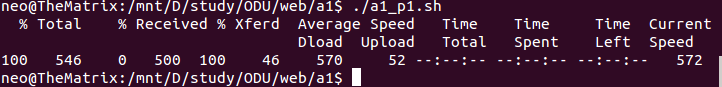
\includegraphics[width=5in]{a1_p1_cmd_response}

\caption{The response in browser}
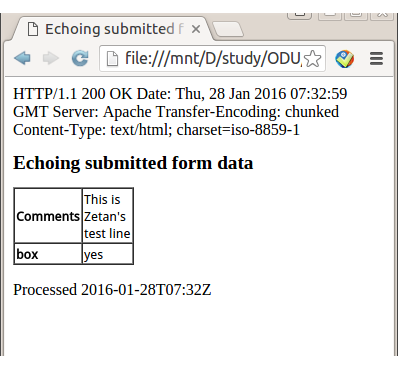
\includegraphics[width=5in]{a1_p1_cresponse}

\end{figure}
\end{homeworkProblem}
\newpage
%----------------------------------------------------------------------------------------
%	PROBLEM 2
%----------------------------------------------------------------------------------------

\begin{homeworkProblem}
Write a Python program that:
  1. takes as a command line argument a web page
  2. extracts all the links from the page
  3. lists all the links that result in PDF files, and prints out
     the bytes for each of the links.  (note: be sure to follow
     all the redirects until the link terminates with a "200 OK".)
  4. show that the program works on 3 different URIs, one of which
     needs to be: 
     http://www.cs.odu.edu/~mln/teaching/cs532-s16/test/pdfs.html
\centerline{SOLUTION}
First, we choose the requests package instead of urllib2. \textbf{requests} can fetch redirect link automatically,
so we don't have to deal with the 300 response in code.\\
Then we are going to read the header of the response, get the value of "Content-type" field, if it's "Application/pdf", then it is a pdf file.\\
The third step is to check whether the link to pdf is available. If so, get the "content-length" field as its size and print the result.
\newpage
\pythonscript{a1_p2}{python script to list the pdf link}
Below is the result of testing \textit{a1\_p2.py} on 3 different URIs:\\
\begin{figure}
\centering
\caption{Test of \textit{a1\_p2.py} at \textbf{http://www.cs.odu.edu/\string~mln/teaching/cs532-s16/test/pdfs.html} }
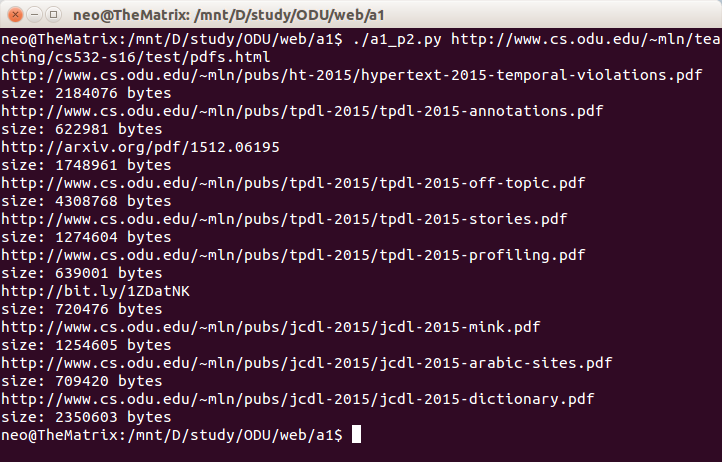
\includegraphics[scale=.5]{a1_p2_result1}

\caption{Test of \textit{a1\_p2.py} at \textbf{http://www.cs.odu.edu} }
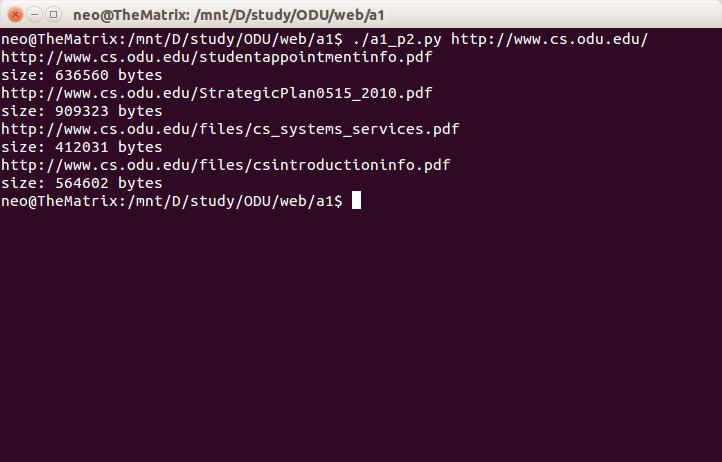
\includegraphics[scale=.5]{a1_p2_result2}
\end{figure}
\newpage
\begin{figure}
\centering
\caption{Test of \textit{a1\_p2.py} at \textbf{http://www.yahoo.com/} }
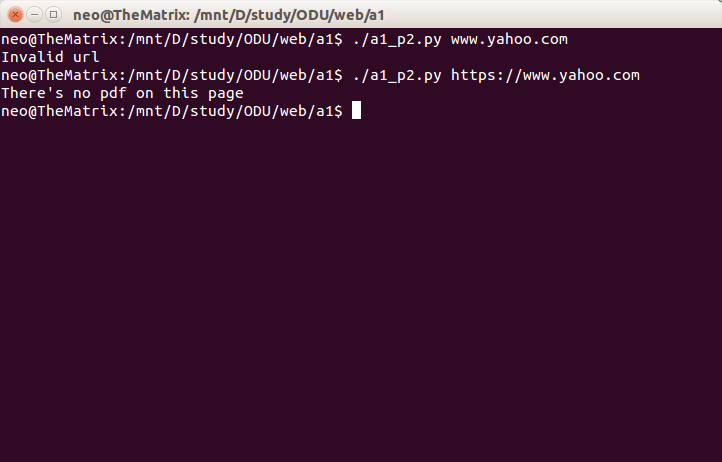
\includegraphics[scale=.5]{a1_p2_result3}
\end{figure}
\end{homeworkProblem}
\newpage
%----------------------------------------------------------------------------------------
%	PROBLEM 3
%----------------------------------------------------------------------------------------

\begin{homeworkProblem}
Consider the "bow-tie" graph in the Broder et al. paper (fig 9):\\
    http://www9.org/w9cdrom/160/160.html\\
\\
    Now consider the following graph:\\
\begin{lstlisting}[frame=single]
    A --> B
    B --> C
    C --> D
    C --> A
    C --> G
    E --> F
    G --> C
    G --> H
    I --> H
    I --> J
    I --> K
    J --> D
    L --> D
    M --> A
    M --> N
    N --> D
    O --> A
    P --> G}
 \end{lstlisting}
    \newpage
    \begin{figure}
\centering
\caption{The bow-tie graph}
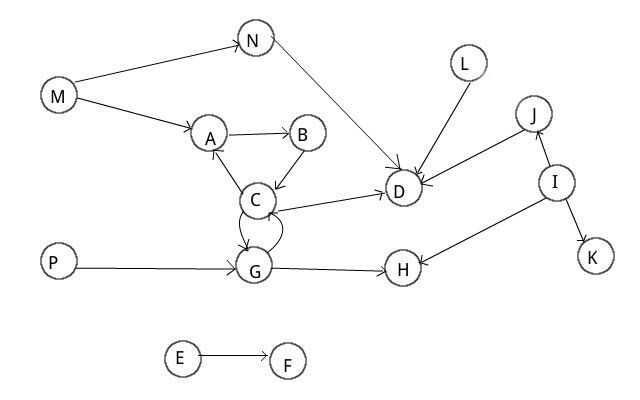
\includegraphics[scale=.5]{a3}
\end{figure}
    For the above graph, give the values for:\\
\\
    IN: \{M,O,P\} The node that can reach the SCC, but can't reach from SCC\\
    SCC: \{A,B,C,G\} The core of the net, every node can reach each other\\
    OUT: \{D,H\}The node that can reach from the SCC, but can't link back to SCC\\
    Tendrils: \{I,J,K,L\}nodes that cannot reach the SCC, and cannot be reached from the SCC\\
    Tubes: \{N\}  A portion of IN to a portion of OUT without touching SCC\\
    Disconnected:\{E,F\} All the other nodes that cannot reach the nodes mentioned above\\
\end{homeworkProblem}
\begin{thebibliography}{9}
\bibitem{Graph structure in the web}
Graph structure in the web. (n.d.) Retrieved January 23, 2016, from \url{http://http://www9.org/w9cdrom/160/160.html}
\end{thebibliography}
\end{document}